\section{The Dilepton $hh \rightarrow \bbww$ Signal Process}
\label{sec:hh_pheno}

In the dilepton channel of the $hh \rightarrow \bbww$ channel, the $WW^*$ system
cannot be fully reconstructed in order to produce, for example, a $WW^*$ invariant
mass observable that has a resonance structure at $m_h = 125$\,GeV.
This is due to the
kinematically under-constrained final state system in which the \met is a result of the double neutrino system
arising from the leptonically decaying $W$ bosons.
Additionally, the final state is the same as that of SM \ttbar~production.
As a result, the dominant SM background to the analysis is expected to be SM \ttbar~and top-quark processes.

There are crucial \textit{topological} differences between the observable final states of dilepton SM \ttbar~production and
that of \bbww, however.
The dileptonic \bbww final state is characterised by `Higgs hemispheres'.
One hemisphere contains the two $b$-tagged jets from the $h \rightarrow bb$ decay and is generally
opposite in the transverse ($xy$) plane to the second hemisphere that contains the two leptons
and \met from the $h \rightarrow WW^*$ decay.
In the case of \ttbar, the $b$-tagged jets, leptons, and neutrinos tend to be distributed more uniformly
within the event, leading to events that do not typically exhibit the same back-to-back hemispheres
topology as the \bbww signal process.
This is illustrated in Figure~\ref{fig:hh_topo}.

The presence of these Higgs hemispheres in the signal, in which the momentum flow of the $WW^*$ system
is correlated with that of the $bb$ system's, will be relied upon to inform the analysis' choice
of kinematic observables that are sensitive to the dilepton $hh \rightarrow \bbww$ signal process.

\begin{figure}[!htb]
    \begin{center}
        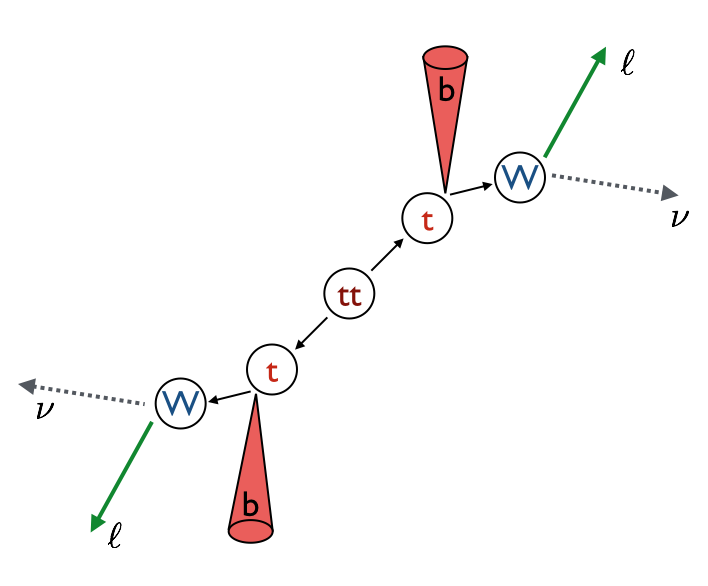
\includegraphics[width=0.52\textwidth]{figures/search_hh/signal_pheno/ttbar_topo}
        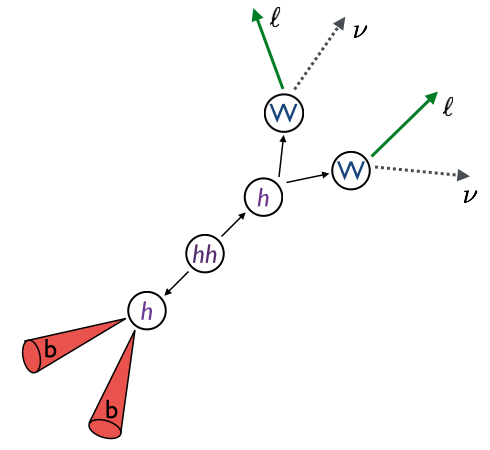
\includegraphics[width=0.46\textwidth]{figures/search_hh/signal_pheno/hh_topo}
        \caption{
            Dilepton $bbWW$ shapes.
            \textit{\textbf{Left}}: SM top-quark pair production.
            \textit{\textbf{Right}}: $hh \rightarrow \bbww$.
        }
        \label{fig:hh_topo}
    \end{center}
\end{figure}

%%%%%%%%%%%%%%%%%%%%%%%%%%%%%%%%%%%%%%%%%%%%%%%%%%%%%%%%%%%%%%%%%%%%%%%%%%%%%%%%%%%
%%%%%%%%%%%%%%%%%%%%%%%%%%%%%%%%%%%%%%%%%%%%%%%%%%%%%%%%%%%%%%%%%%%%%%%%%%%%%%%%%%%
%%%%%%%%%%%%%%%%%%%%%%%%%%%%%%%%%%%%%%%%%%%%%%%%%%%%%%%%%%%%%%%%%%%%%%%%%%%%%%%%%%%
%
% KINEMATIC DISTRIBUTIONS/SHAPES
%
%%%%%%%%%%%%%%%%%%%%%%%%%%%%%%%%%%%%%%%%%%%%%%%%%%%%%%%%%%%%%%%%%%%%%%%%%%%%%%%%%%%
%%%%%%%%%%%%%%%%%%%%%%%%%%%%%%%%%%%%%%%%%%%%%%%%%%%%%%%%%%%%%%%%%%%%%%%%%%%%%%%%%%%
%%%%%%%%%%%%%%%%%%%%%%%%%%%%%%%%%%%%%%%%%%%%%%%%%%%%%%%%%%%%%%%%%%%%%%%%%%%%%%%%%%%

In the following we present some kinematic distributions illustrating the unique topologies
of the dilepton $hh \rightarrow \bbww$ signal process as compared to the dominant top-quark background
processes.

Figure~\ref{fig:hh_kin_0} shows distributions related to the $bb$ system.
It can be seen from the $|\Delta \phi|$ and $\Delta R$ distributions that the two $b$-tagged jets
are collinear in the signal process as compared to the background processes.
For the \ttbar background, these tendencies in $|\Delta \phi|$ and $\Delta R$ are reversed,
as expected from their different topology with the $b$-tagged jets on opposing sides of the event.
For single-top $Wt$, similar trends as observed in \ttbar are observe but, since the second $b$-tagged
jet in the $Wt$ process is due to higher-order contributions (or a light-flavor jet mistakenly identified as a $b$-jet),
the $b$-tagged jets are often more collinear.

Figure~\ref{fig:hh_kin_1} shows a few distributions related to the dilepton, \met, and $\met$ + dilepton systems.
We can see from the $|\Delta \phi|$ and $\Delta R$ distributions that for the signal $hh$ process, the leptons
are collinear as expected, with the leptons contained almost entirely within a cone of radius $\Delta R = 1$.
For the top-quark backgrounds, there is a tendency for the leptons to be back-to-back, with $|\Delta \phi| (\Delta R) \rightarrow \pi$.

The $|\Delta \phi|$ between the \met and dilepton system, $|\dphimetll|$, shows that the $WW^*$ system is collinear, as well.
For the SM top-quark backgrounds, $|\dphimetll|$ tends slowly towards $\pi$.
In the case of single-top $Wt$, however, there is a tendency for $|\dphimetll|$ to gather towards lower values due
to similar effects as described previously: the more collinear $b$-tagged jets force the
$WW^*$ system to also become collinear so that it balances the $bb$ system.

\begin{figure}[!htb]
    \begin{center}
        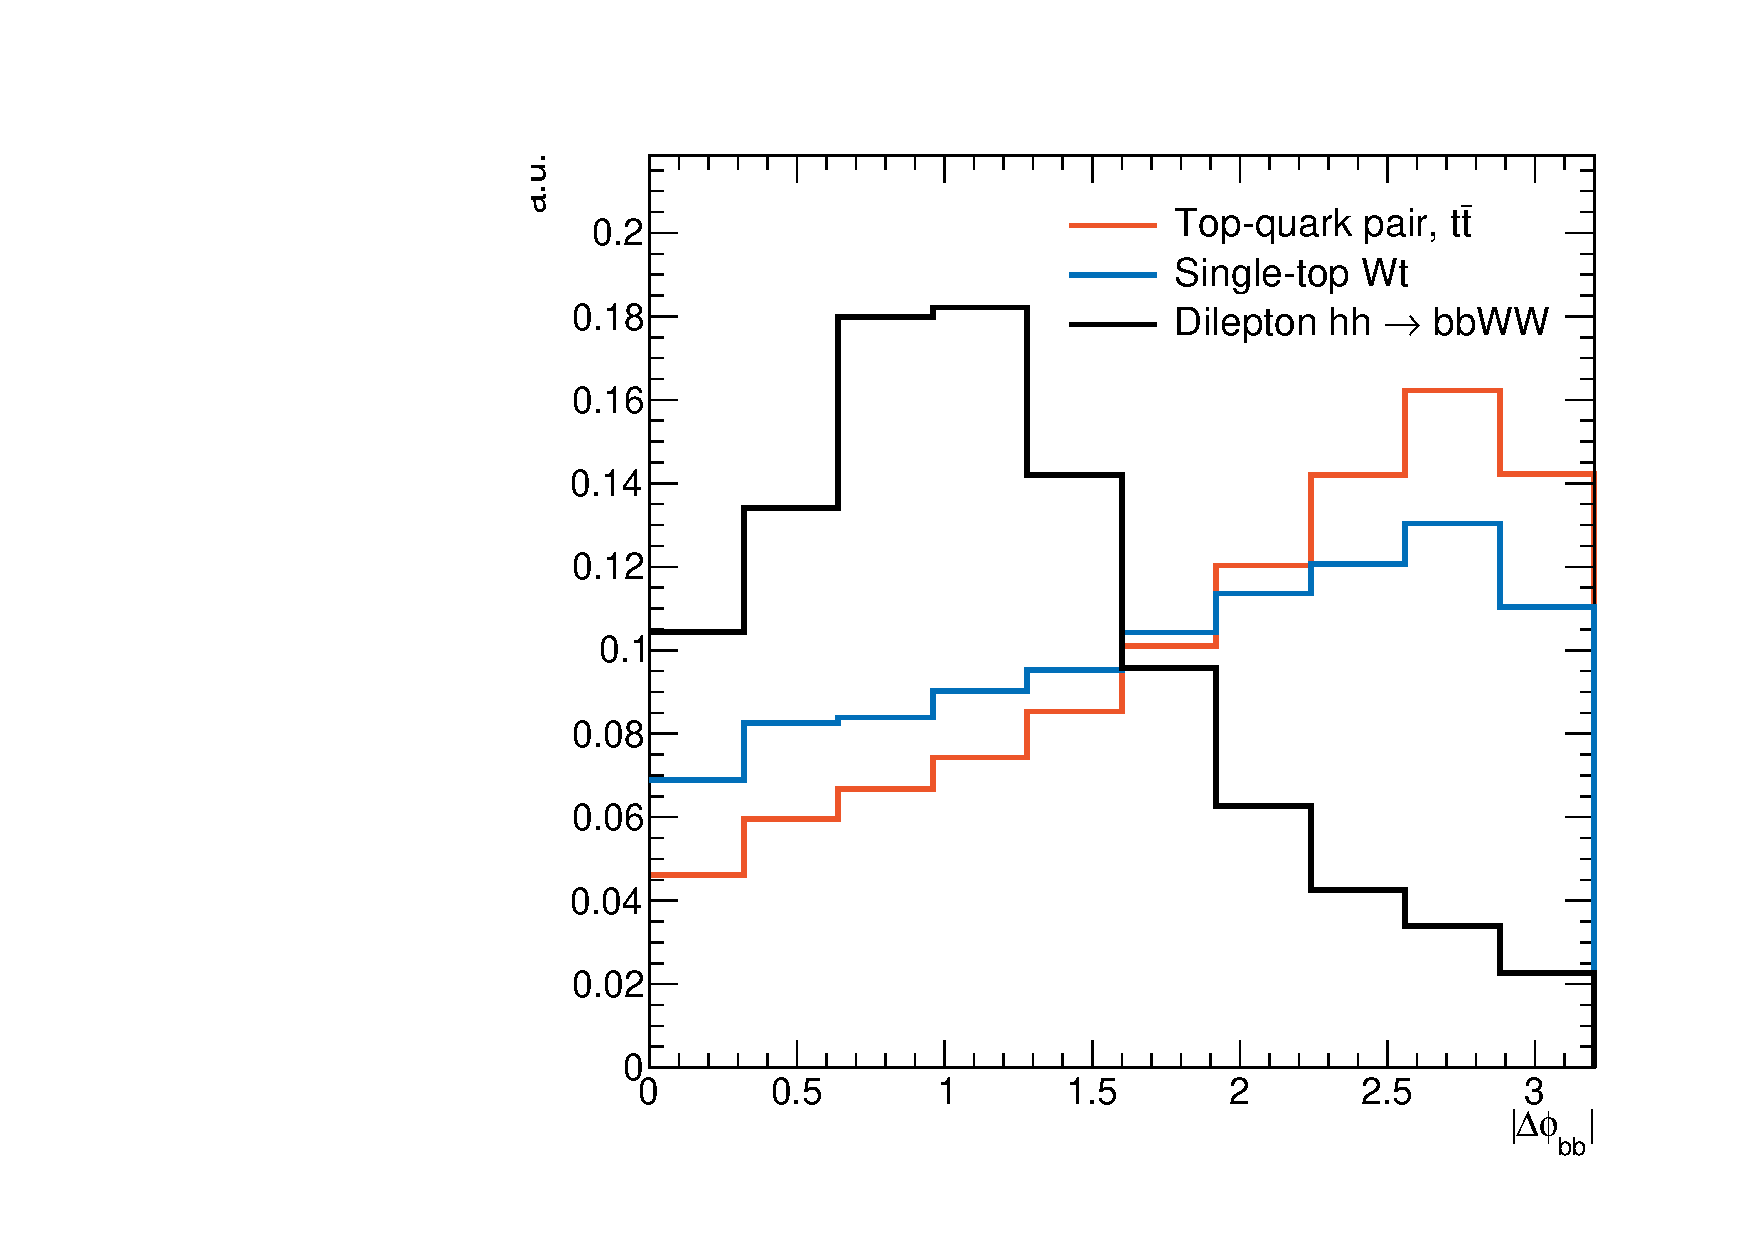
\includegraphics[width=0.45\textwidth]{figures/search_hh/signal_pheno/shape_plots/hh_shape_plot_dphi_bb}
        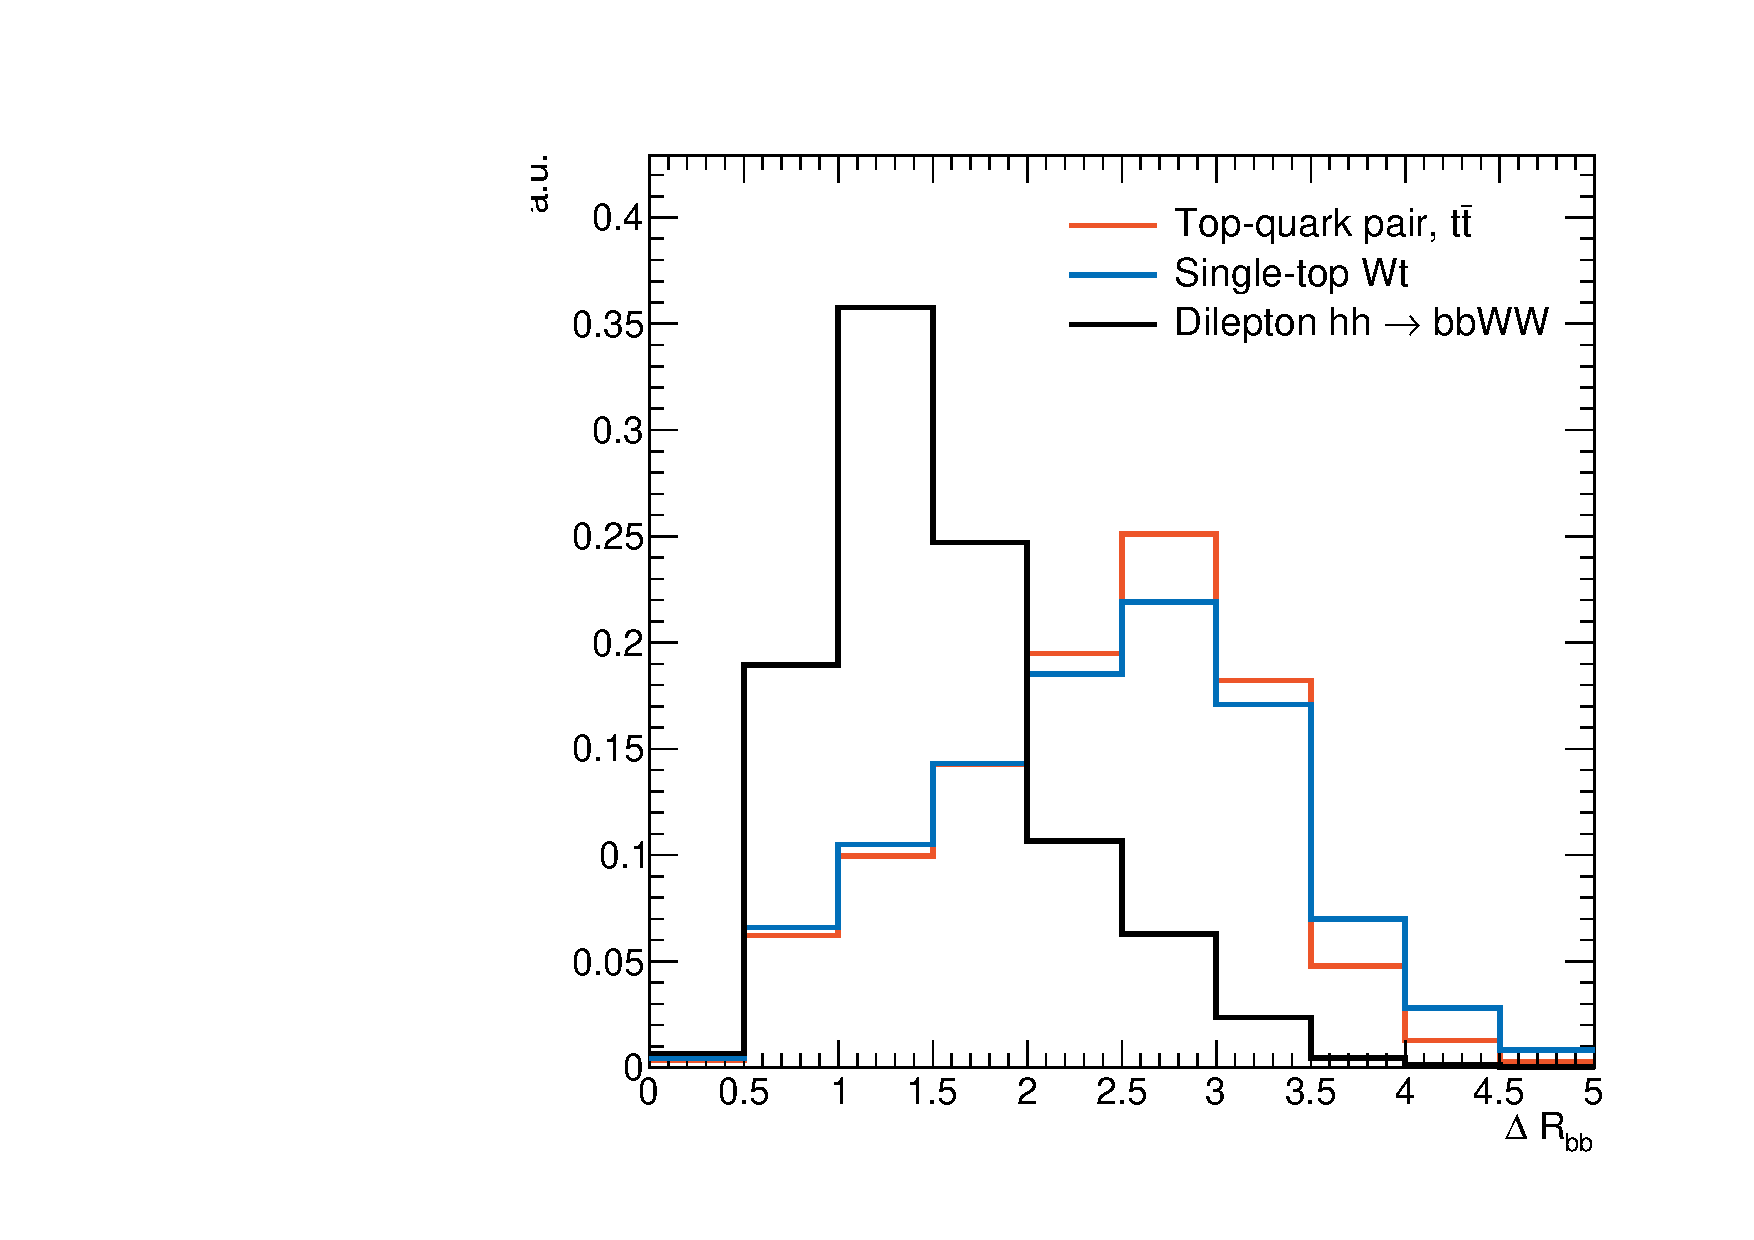
\includegraphics[width=0.45\textwidth]{figures/search_hh/signal_pheno/shape_plots/hh_shape_plot_dRbb}
        \caption{
            Normalized distributions showing the shapes of kinematic distributions for the SM
            top-quark processes (\ttbar~and single-top $Wt$) and the dilepton $hh \rightarrow \bbww$ signal process.
            \textit{\textbf{Left}}: $|\Delta \phi|$ between the two $b$-tagged jets.
            \textit{\textbf{Right}}: $\Delta R$ between the two $b$-tagged jets.
        }
        \label{fig:hh_kin_0}
    \end{center}
\end{figure}

\begin{figure}[!htb]
    \begin{center}
        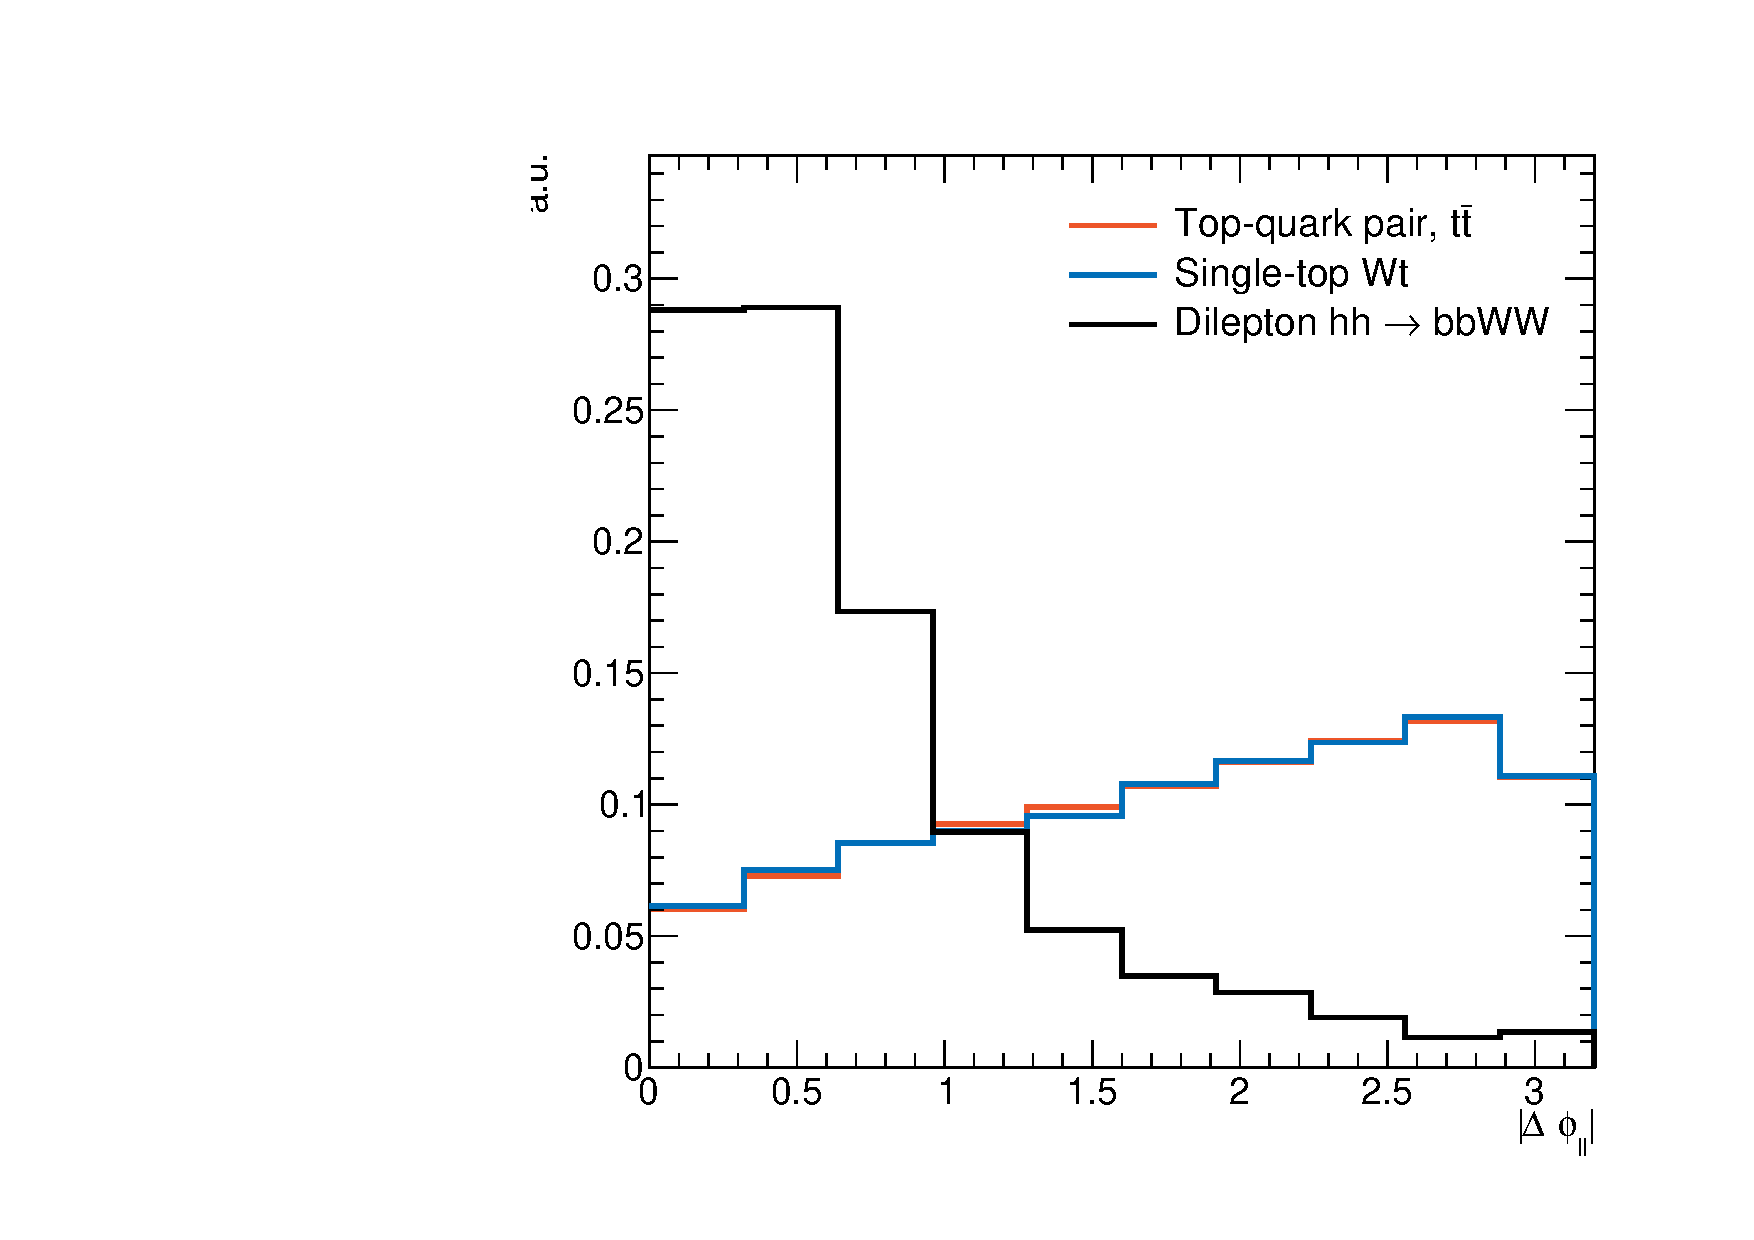
\includegraphics[width=0.45\textwidth]{figures/search_hh/signal_pheno/shape_plots/hh_shape_plot_dphi_ll}
        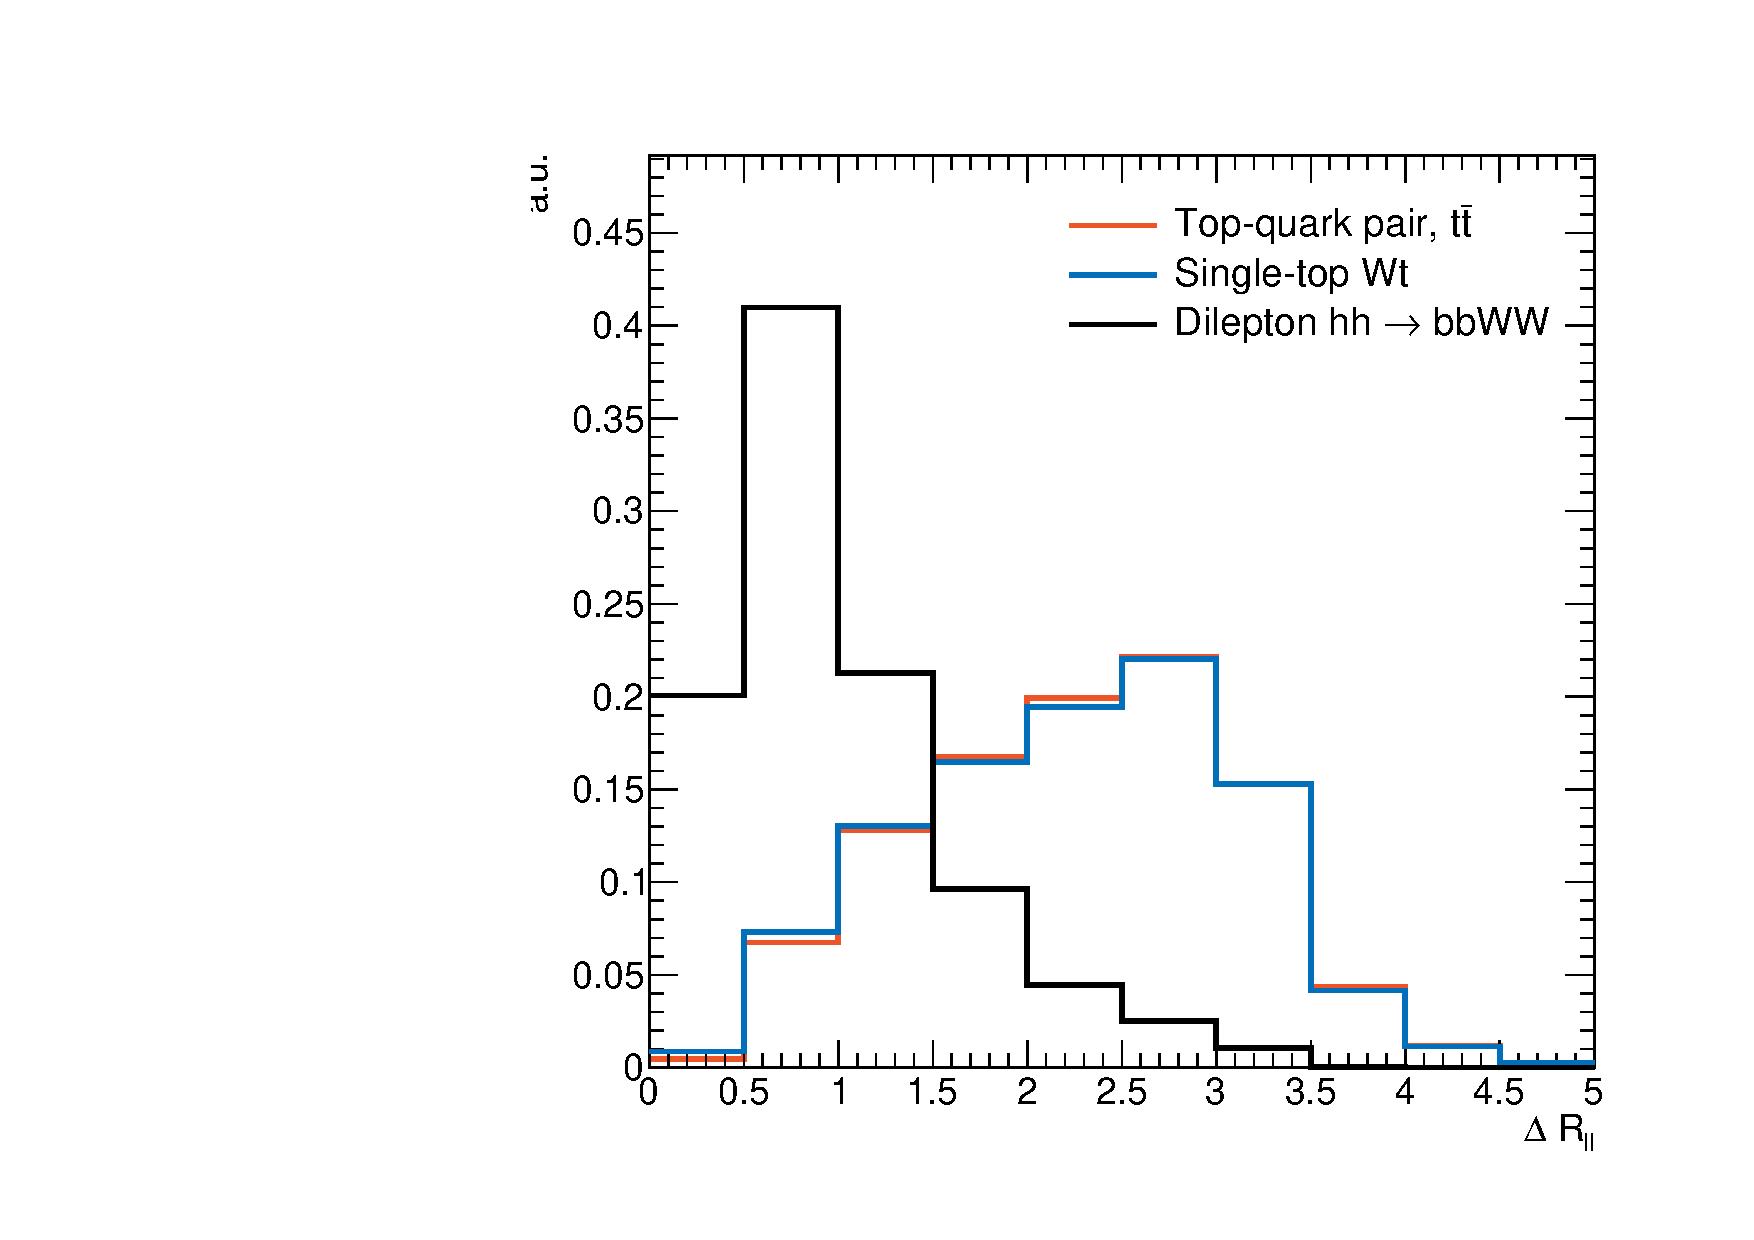
\includegraphics[width=0.45\textwidth]{figures/search_hh/signal_pheno/shape_plots/hh_shape_plot_dRll}
        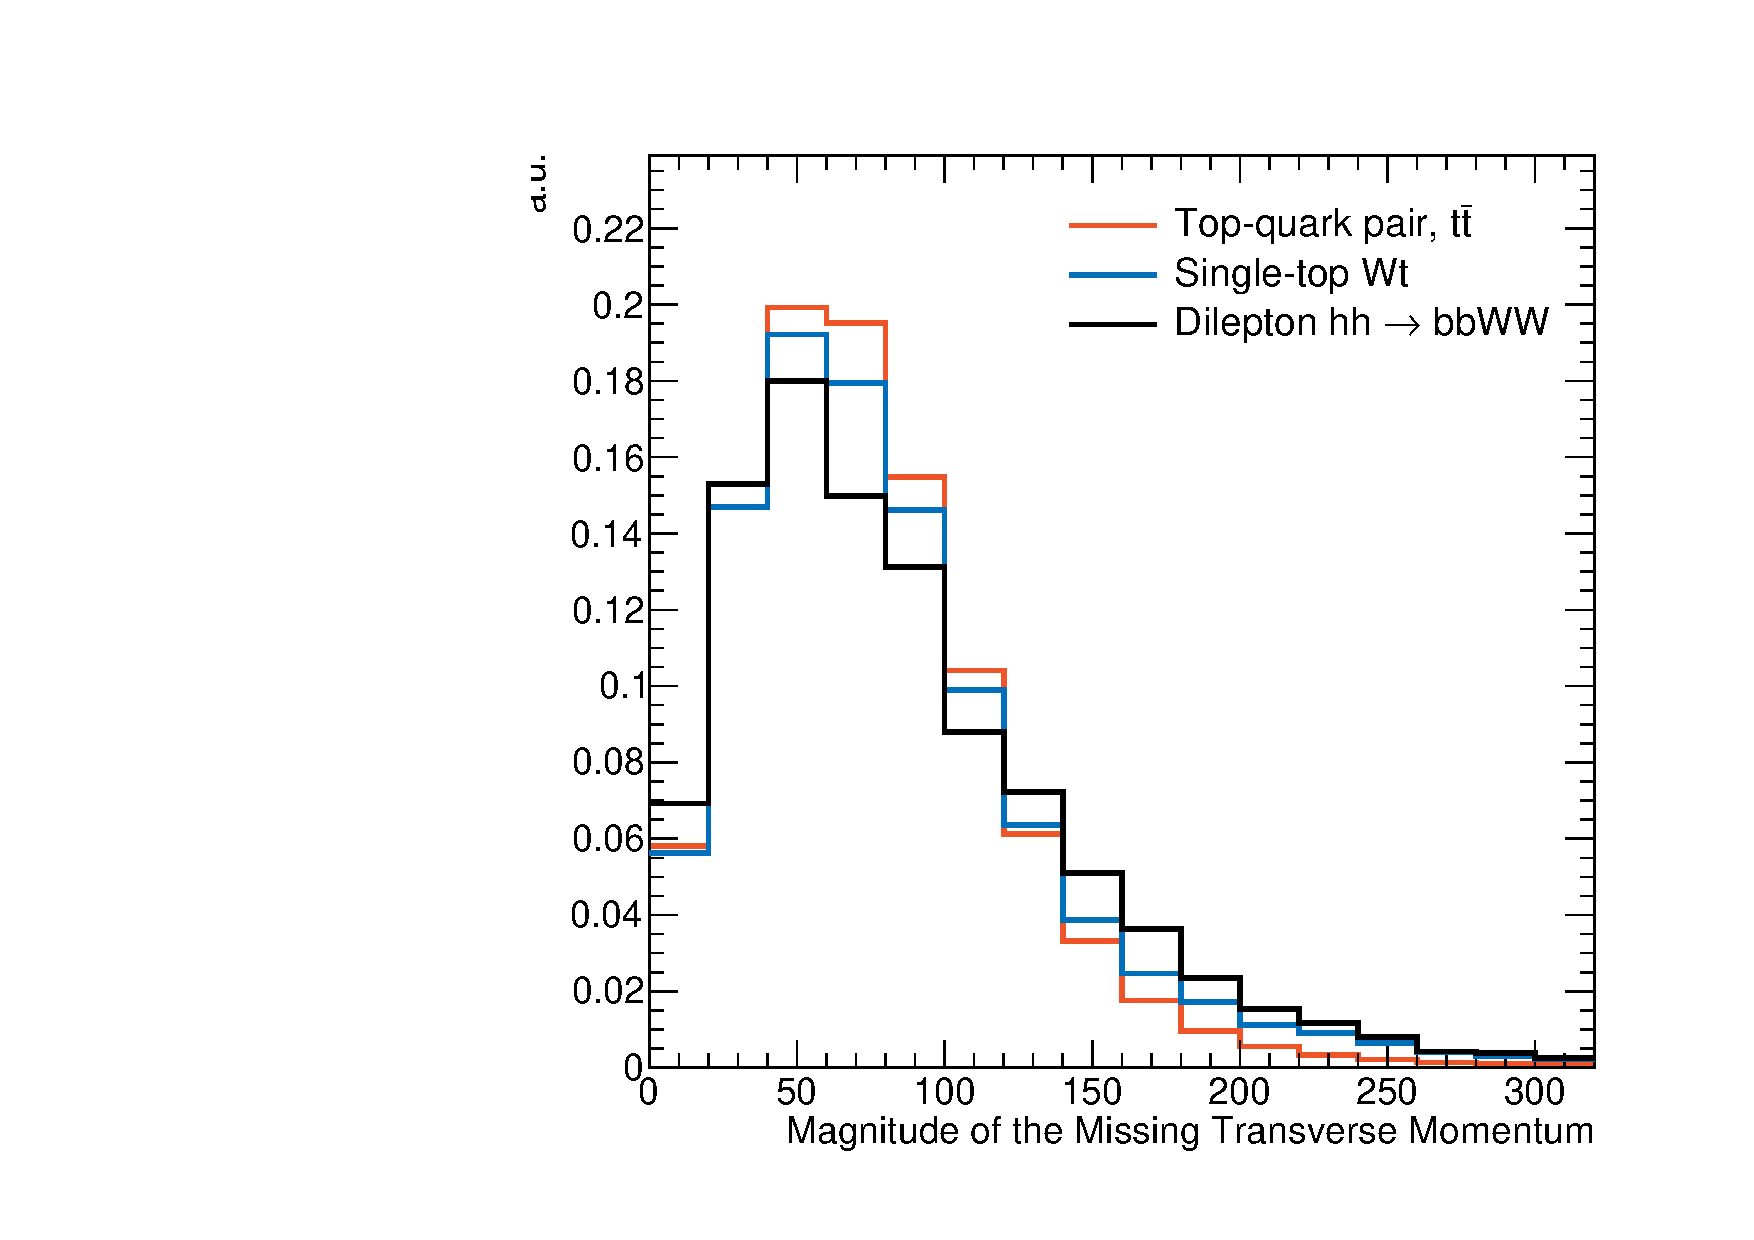
\includegraphics[width=0.45\textwidth]{figures/search_hh/signal_pheno/shape_plots/hh_shape_plot_met}
        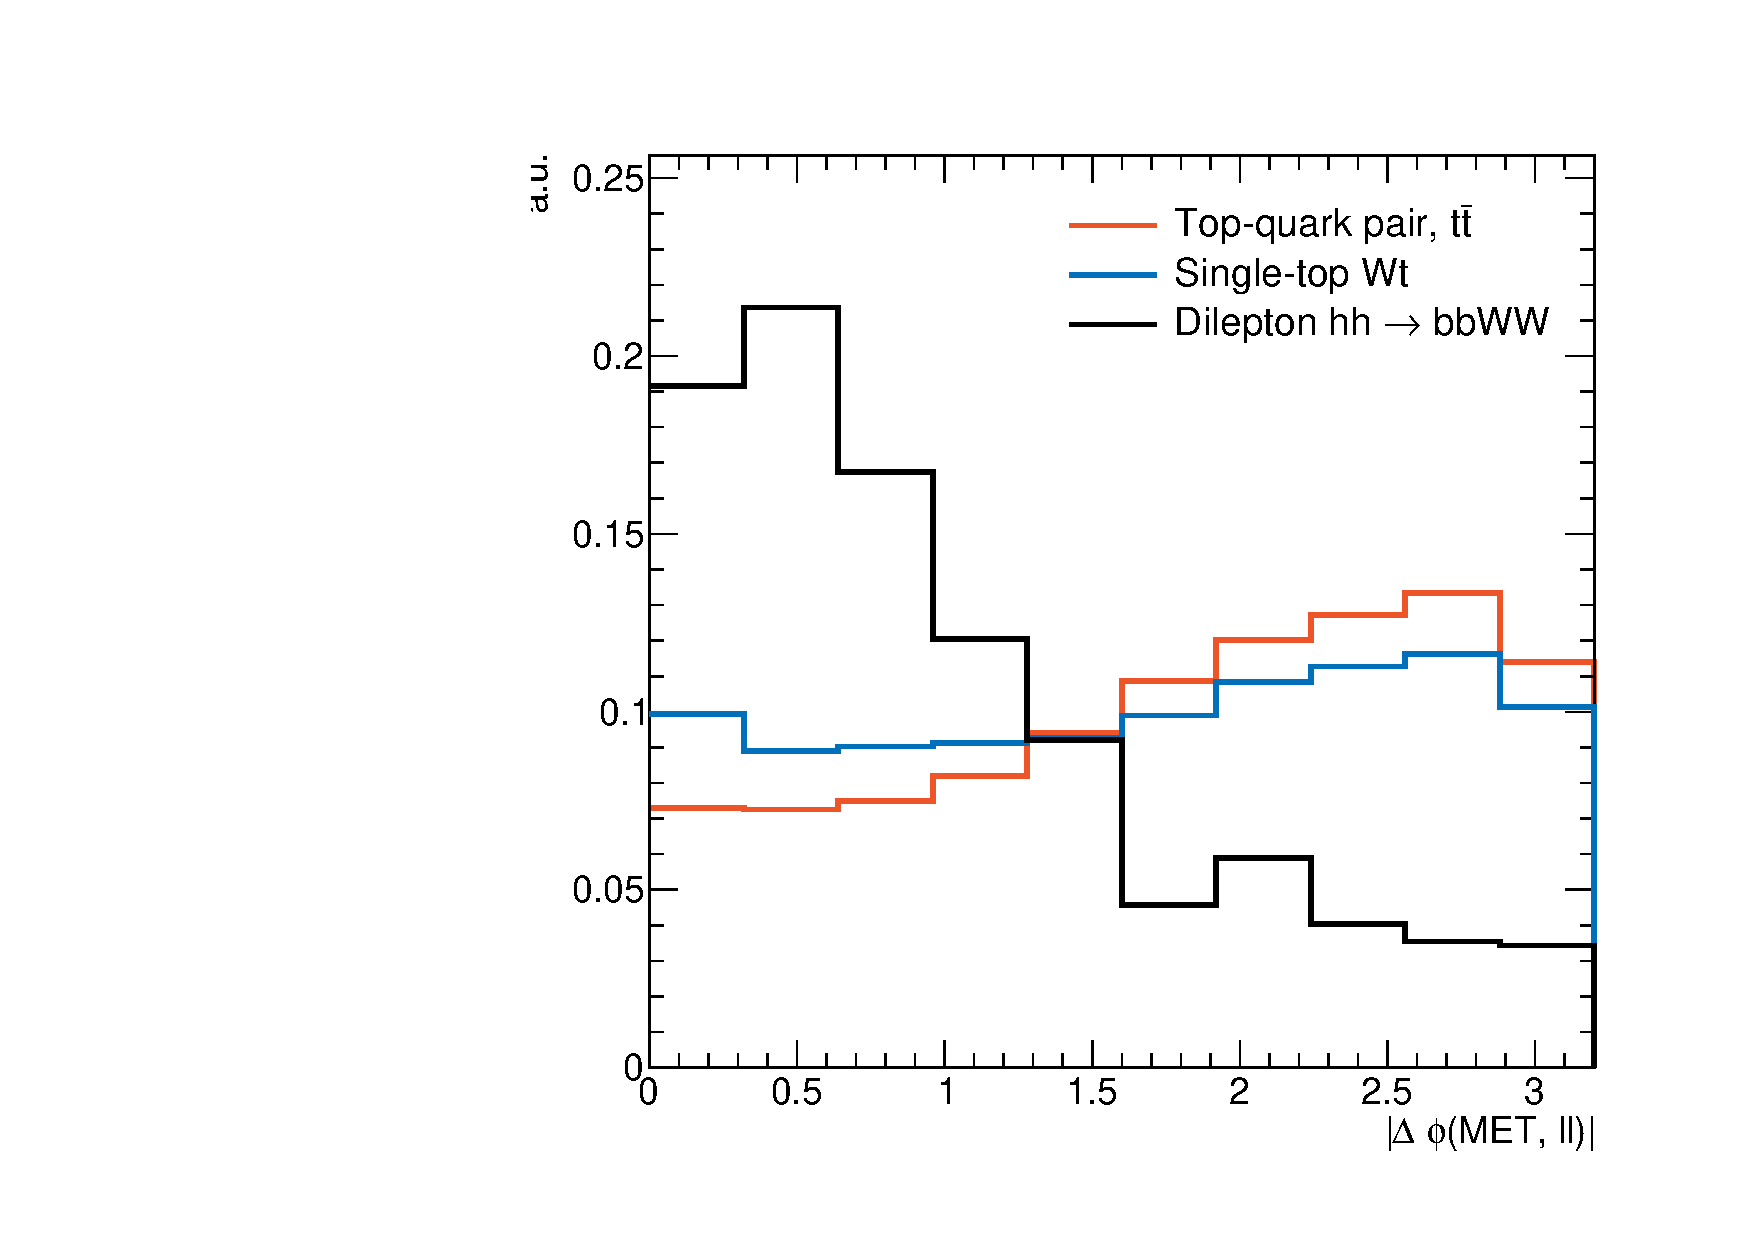
\includegraphics[width=0.45\textwidth]{figures/search_hh/signal_pheno/shape_plots/hh_shape_plot_dphi_met_ll}
        \caption{
            Normalized distributions showing the shapes of kinematic distributions for the SM
            top-quark processes (\ttbar~and single-top $Wt$) and the dilepton $hh \rightarrow \bbww$ signal process.
            \textit{\textbf{Left, upper}}: $|\Delta \phi|$ between the two leptons.
            \textit{\textbf{Right, upper}}: $\Delta R$ between the two leptons.
            \textit{\textbf{Left, lower}}: $\met$.
            \textit{\textbf{Right, lower}}: $\Delta \phi$ between \met and dilepton system.
        }
        \label{fig:hh_kin_1}
    \end{center}
\end{figure}

%%%%%%%%%%%%%%%%%%%%%%%%%%%%%%%%%%%%%%%%%%%%%%%%%%%%%%%%%%%%%%%%%%%%%%%%%%%%%%%%%%%
%%%%%%%%%%%%%%%%%%%%%%%%%%%%%%%%%%%%%%%%%%%%%%%%%%%%%%%%%%%%%%%%%%%%%%%%%%%%%%%%%%%
%%%%%%%%%%%%%%%%%%%%%%%%%%%%%%%%%%%%%%%%%%%%%%%%%%%%%%%%%%%%%%%%%%%%%%%%%%%%%%%%%%%
%
% TARGETTED OBSERVABLES
%
%%%%%%%%%%%%%%%%%%%%%%%%%%%%%%%%%%%%%%%%%%%%%%%%%%%%%%%%%%%%%%%%%%%%%%%%%%%%%%%%%%%
%%%%%%%%%%%%%%%%%%%%%%%%%%%%%%%%%%%%%%%%%%%%%%%%%%%%%%%%%%%%%%%%%%%%%%%%%%%%%%%%%%%
%%%%%%%%%%%%%%%%%%%%%%%%%%%%%%%%%%%%%%%%%%%%%%%%%%%%%%%%%%%%%%%%%%%%%%%%%%%%%%%%%%%

To take further advantage of the topological differences mentioned in the preceding, we can construct
an observable that is sensitive to the overall distribution of the momentum flow in the event.
This is to capture the more `planar' nature of the dilepton $hh \rightarrow \bbww$ decay as compared
to that of the SM top-quark backgrounds.
This observable, \htratio, is defined as follows,
\begin{align}
    \htratio &= \frac{\htnum}{\htden},
    \label{eq:ht2ratio_def}
\end{align}
where the $\bm{p}_{\text{T}}^{\ell(b),0 \{1\}}$ are the transverse momenta of the leading \{subleading\} lepton ($b$-tagged jet).

The numerator of Equation~\ref{eq:ht2ratio_def} contains two parts, each the magnitude of a vectorial sum of transverse
momenta: the first part containing the objects associated with the $WW^*$ decay and the second with those associated
with the $bb$ decay.
For the dilepton $hh \rightarrow \bbww$ signal, then, the numerator is the sum of the magnitudes of each of the Higgs boson's
momenta.
The denominator appearing in Equation~\ref{eq:ht2ratio_def} is the scalar sum of the transverse momenta of each of the
final state objects considered in teh analysis.
By taking this ratio, a measure of the overall spread of the momentum in the event is obtained.

For the relevant SM top-quark processes, with the visible final state objects distributed more evenly
about the event, the quantities appearing in the numerator of Equation~\ref{eq:ht2ratio_def} will
tend to be smaller, due to vectorial cancellation, than in the case of the $hh$ signal.
Due to the Higgs hemispheres in the signal, with separately collinear $WW^*$ and $bb$ systems,
the numerator in Equation~\ref{eq:ht2ratio_def} will be large.
It follows, then, that the quantity \htratio should tend towards unity for the dilepton $hh \rightarrow \bbww$
signal process and towards lower values for the SM top-quark processes.
This behavior is illustrated in Figure~\ref{fig:hh_shape_htratio}.

\begin{figure}[!htb]
    \begin{center}
        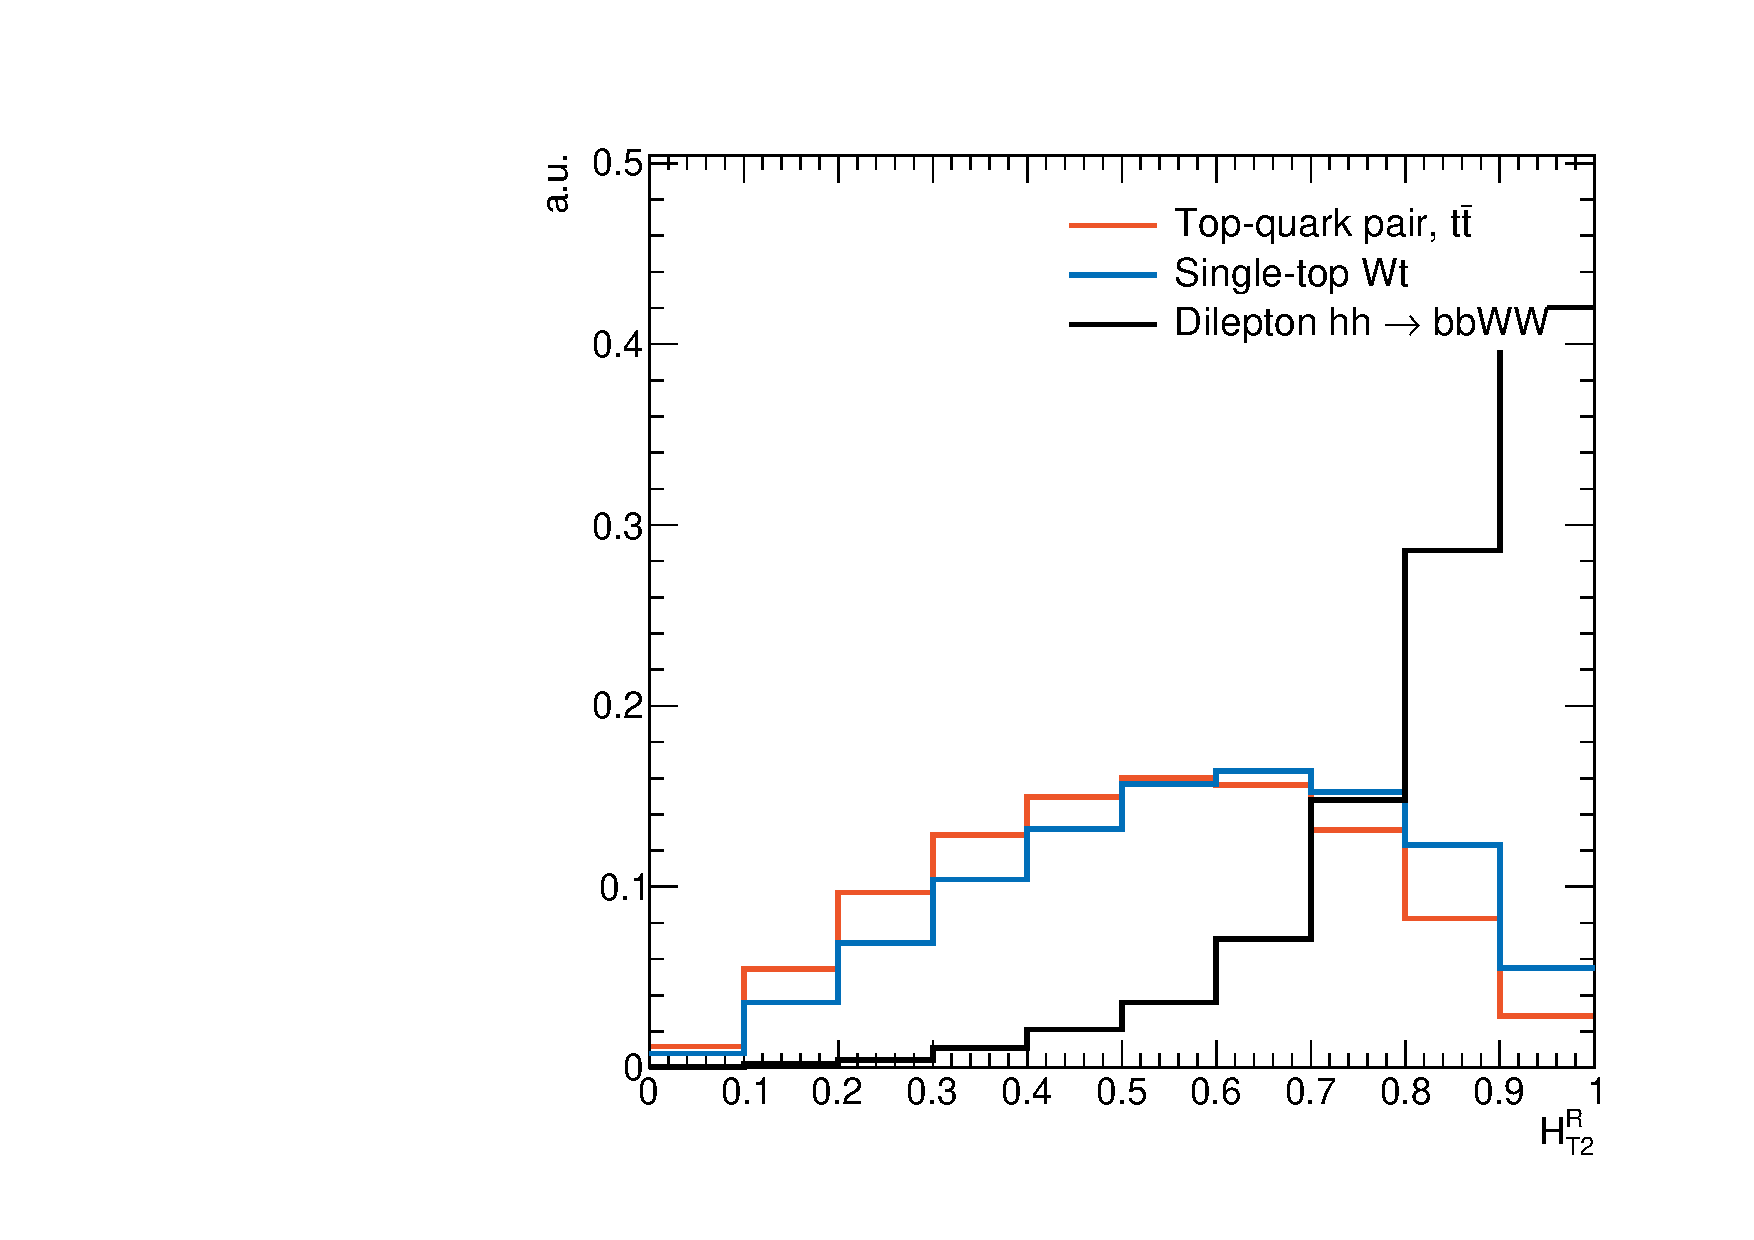
\includegraphics[width=0.6\textwidth]{figures/search_hh/signal_pheno/shape_plots/hh_shape_plot_HT2Ratio}
        \caption{
            Normalized distributions showing the shape of the \htratio observable for the SM
            top-quark processes (\ttbar~and single-top $Wt$) and the dilepton $hh \rightarrow \bbww$ signal process.
        }
        \label{fig:hh_shape_htratio}
    \end{center}
\end{figure}

We also consider a variant of the \mttwo variable~\cite{MT2-Glamour,Lester2011,MT2-Tovey-Masses,Lester2014yga},
a transverse-mass variable that can be used in events where there are two or more invisible particles,
as is our case with the two neutrinos.
Generally, \mttwo assumes that the decay is symemtric, as in \ttbar, where there are two decay legs, each with
a visible and invisible child particle decay.
The \mttwo observable is generically defined as follows,
\begin{align}
    \mttwo^2 \equiv \min\limits_{ \bm{q}_{\text{T}}^{\text{miss},\,a} + \, \bm{q}_{\text{T}}^{\text{miss},\,b} = \,\bm{p}_{\text{T}}^{\text{miss}}}
        \left[
            \max
                \left\{
                    m_{\text{T}}^2 ( \bm{p}_{\text{T}}^{\text{vis},\, a}, \bm{q}_{\text{T}}^{\text{miss},\,a} ), m_{\text{T}}^2 (\bm{p}_{\text{T}}^{\text{vis},\, b}, \bm{q}_{\text{T}}^{\text{miss},\,b} )
                \right\}
        \right],
    \label{eq:mttwo_def}
\end{align}
where `a' (`b') indicate one of the two sides of the decay and the $\bm{p}_{\text{T}}^i$ are the transverse momenta
of the visible objects on side $i \in (a,b)$, and $\bm{q}_{\text{T}}^i$ is a partition of the total \ptmiss given to side $i \in (a,b)$.
The minimization is carried out over all partionings of the \ptmiss into the $\bm{q}_{\text{T}}^i$ and the $m_{\text{T}}$ are the typical
transverse masses,
\begin{align}
    m_{\text{T}}^2 (\bm{p}_{\text{T}}^{\text{vis}}, \bm{q}_{\text{T}}^{\text{miss}} ) = ( E_{\text{T}}^{\text{vis}} + | \bm{q}_{\text{T}}^{\text{miss}} |)^2
            - |\bm{p}_{\text{T}}^{\text{vis}} + \bm{q}_{\text{T}}^{\text{miss}} |^2
    \label{eq:mt_def}
\end{align}

The \mttwo-based observable defined for the present analysis is referred to as `\mtbb',
and is an \mttwo construction in which the visible objects are the two $b$-tagged jets in the event.
This means that side `a' (`b'), using the notation of Equation~\ref{eq:mttwo_def}, contains
one of the $b$-tagged jets as $\bm{p}_{\text{T}}^{\text{vis, a}}$ ($\bm{p}_{\text{T}}^{\text{vis}, b}$).

Given the fact that in the SM top-quark backgrounds, the neutrinos (approximated by the $\bm{q}_{\text{T}}^{\text{miss}, i}$)
and the $b$-tagged jets originate from the same origin (a top-quark), the \mtbb observable tends
to have a kinematic bound at roughly the mass of the top-quark, $m_{\text{top}}$.
In the SM \ttbar~process, where both $b$-tagged jets originate from the decay of a top-quark, this kinematic
endpoint is strict.
In the case of single-top $Wt$, however, where only one $b$-tagged jet arises from the decay of a
top-quark, the \mtbb observable can extend beyond $m_{\text{top}}$.
Figure~\ref{fig:hh_shape_mtbb} illustrates the \mtbb observable.

\begin{figure}[!htb]
    \begin{center}
        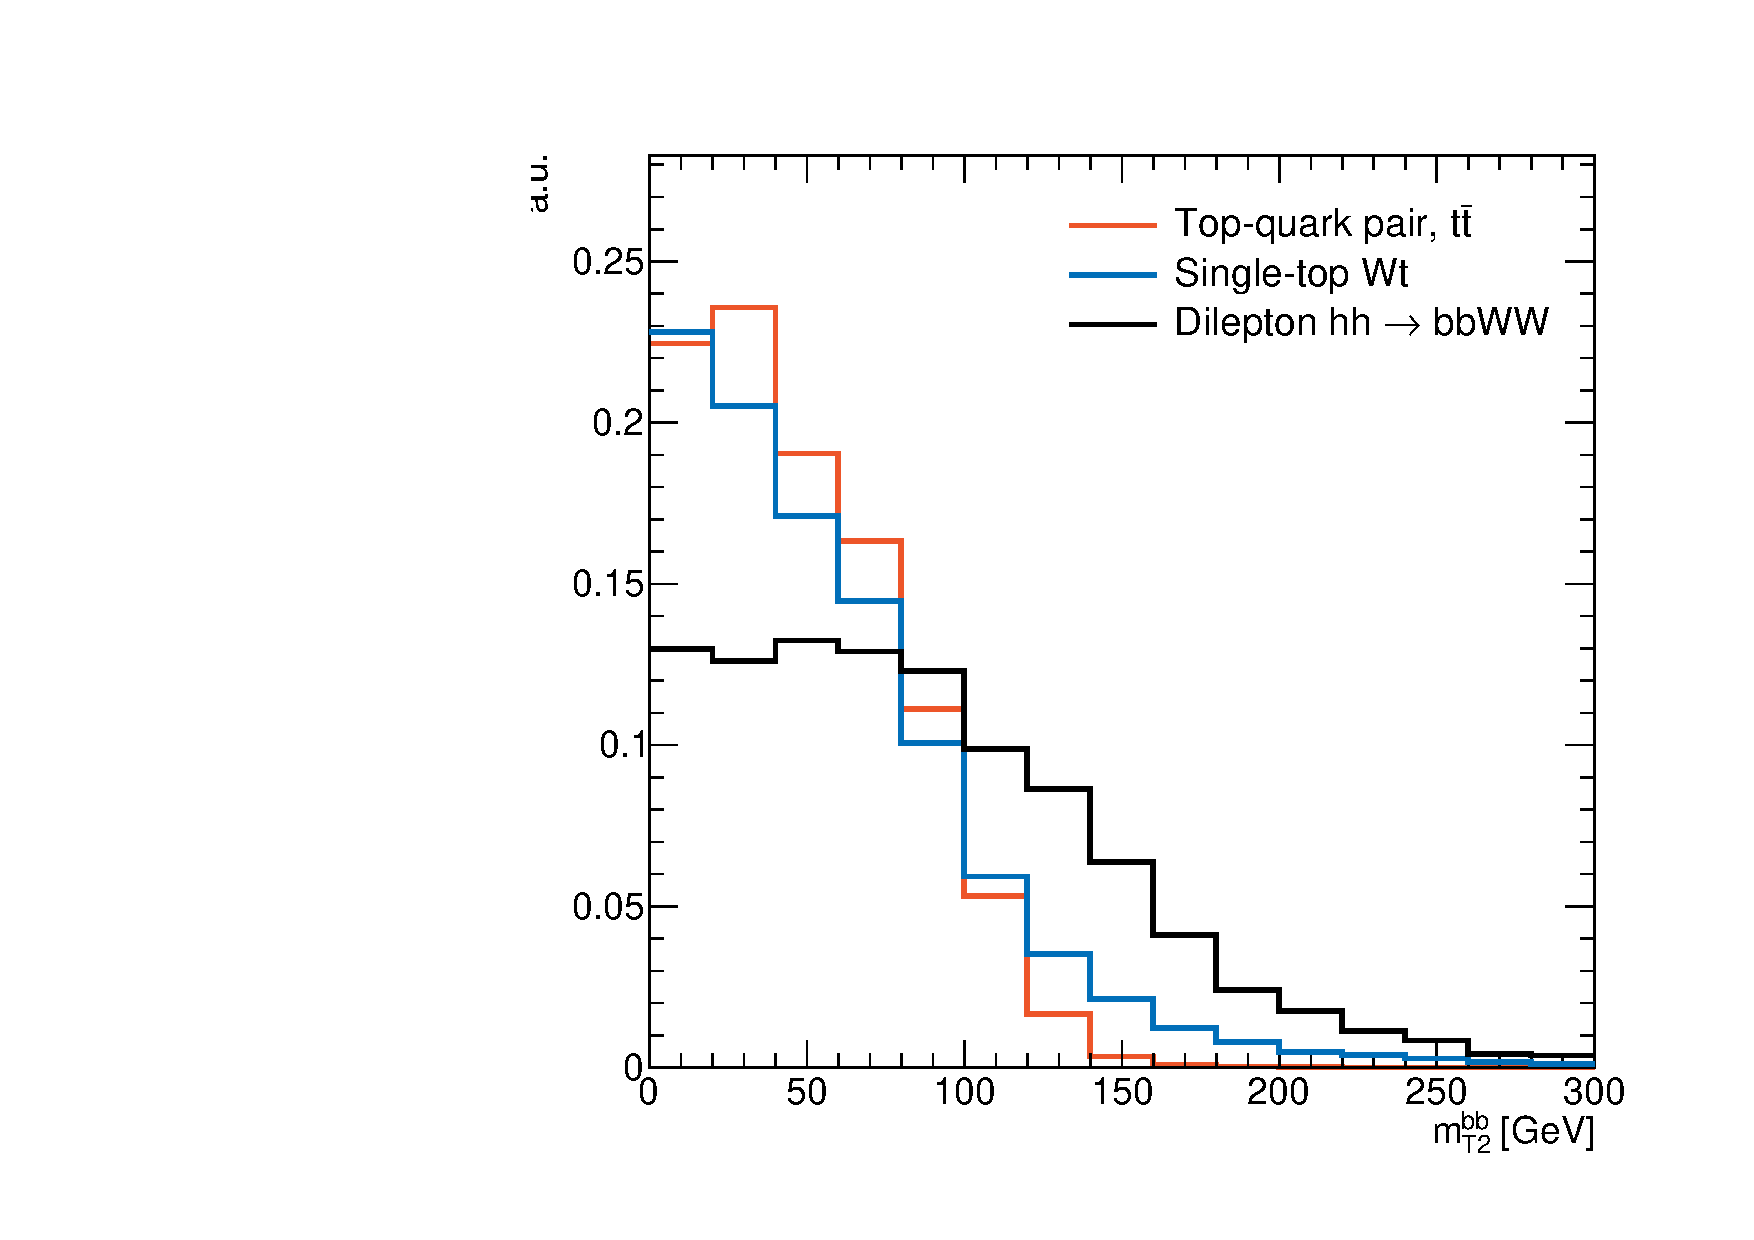
\includegraphics[width=0.6\textwidth]{figures/search_hh/signal_pheno/shape_plots/hh_shape_plot_mt2_bb}
        \caption{
            Normalized distributions showing the shape of the \mtbb observable for the SM
            top-quark processes (\ttbar~and single-top $Wt$) and the dilepton $hh \rightarrow \bbww$ signal process.
        }
        \label{fig:hh_shape_mtbb}
    \end{center}
\end{figure}


